%%%%%%%%%%%%%%%%%%%%%%%%%%%%%%%%%%%%% 
%% LE2I beamer template
%% Guillaume Lemaitre, October 2014
%%%%%%%%%%%%%%%%%%%%%%%%%%%%%%%%%%%%% 

\documentclass{beamer}

\usepackage[utf8]{inputenc}
\usepackage[T1]{fontenc} 
\usetheme{le2i} 

%% The amssymb package provides various useful mathematical symbols
\usepackage{amssymb}
%% The amsthm package provides extended theorem environments
\usepackage{amsthm}
%% amsmath for math environment
\usepackage{amsmath}

\DeclareMathOperator*{\argmin}{arg\,min}
\DeclareMathOperator*{\argmax}{arg\,max}
\DeclareMathOperator*{\sign}{sign}

%% figure package
\usepackage{epsf,graphicx}
\usepackage{epstopdf}
\usepackage{subfigure}
\usepackage{transparent}

%% In order to draw some graphs
\usepackage{tikz,xifthen}
\usepackage{tikz-qtree}
\usepackage{adjustbox}
\usetikzlibrary{decorations.pathmorphing}
\usetikzlibrary{fit}
\usetikzlibrary{backgrounds}
\usetikzlibrary{shapes,arrows,shadows}
\usetikzlibrary{calc,decorations.pathreplacing,decorations.markings,positioning}
\usetikzlibrary{snakes,decorations.text,shapes,patterns}
% \usepackage{scalefnt,lmodern,booktabs}

%% Package for cross and tick symbols
\usepackage{pifont}
\newcommand{\tick}{\color{green!60!black!80}\ding{51}}
\newcommand{\cross}{\color{red!60!black!80}\ding{55}}

\setbeamercovered{transparent}
\resetcounteronoverlays{subfigure}

\usepackage{biblatex}
\addbibresource{bibtex.bib}

\title{\Large{A Boosting Approach for Prostate Cancer Detection using Multi-Parametric MRI}}
\author{\scriptsize{Guillaume Lemaitre \\ \texttt{guillaume.lemaitre@u-bourgogne.fr}}}
\date{\scriptsize{Quality Control by Artificial Vision \\ 4\textsuperscript{th} June 2015}}

\institute{Universit\'e de Bourgogne} 

\newenvironment<>{redblock}[1]{%
  \begin{actionenv}#2%
    \def\insertblocktitle{#1}%
    \par%
    \mode<presentation>{%
      \setbeamercolor{block title}{fg=nicewhite,bg=red!75!black}
      \setbeamercolor{block body}{fg=niceblack,bg=red!20}
    }%
    \usebeamertemplate{block begin}}
  {\par\usebeamertemplate{block end}\end{actionenv}}

\newenvironment<>{greenblock}[1]{%
  \begin{actionenv}#2%
    \def\insertblocktitle{#1}%
    \par%
    \mode<presentation>{%
      \setbeamercolor{block title}{fg=nicewhite,bg=green!40!black}
      \setbeamercolor{block body}{fg=niceblack,bg=green!20}
    }%
    \usebeamertemplate{block begin}}
  {\par\usebeamertemplate{block end}\end{actionenv}}

%% Uncomment if you want to avoid thousand of bullet inside the menu
% \usepackage{etoolbox}
% \makeatletter
% \patchcmd{\slideentry}{\advance\beamer@xpos by1\relax}{}{}{}
% \def\beamer@subsectionentry#1#2#3#4#5{\advance\beamer@xpos by1\relax}%
% \makeatother

\begin{document}

% Show the title page
\begin{frame}
  \titlepage
\end{frame}

% Show the table of contents
\begin{frame}
  \tableofcontents[sectionstyle=show,subsectionstyle=show,subsubsectionstyle=hide]
\end{frame}

\section{Introduction}

\subsection{Motivations}

\begin{frame}
  \frametitle{Introduction}
  \framesubtitle{Motivations}
  \begin{block}{\small Statistics}
    \begin{figure}%
      \centering
      \hspace*{\fill}%
      \subfigure[][\tiny \# of cancer cases]{%
        \label{fig:stat1a}%
          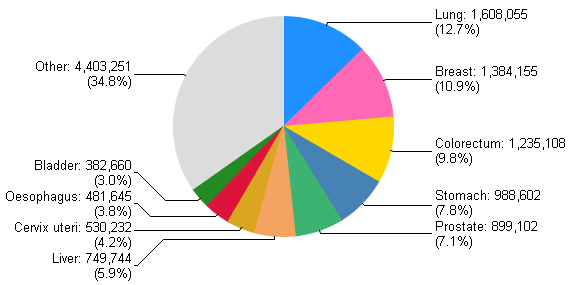
\includegraphics[width=.45\textwidth]{./images/statistics/repartitionCancerIncidence.png}}%
      \hfill%
      \subfigure[][\tiny \# of cancer deaths]{%
        \label{fig:stat1b}%
          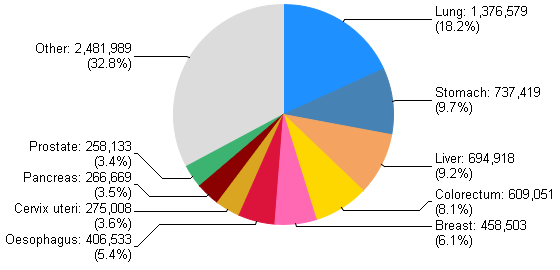
\includegraphics[width=.45\textwidth]{./images/statistics/repartitionCancerDeaths.png}}%
        \hspace*{\fill}%
      \label{fig:stat1}%
    \end{figure}
  \end{block}
  \begin{block}<2->{\small Implications}\footnotesize
    \begin{itemize}
    \item<2-> 2\textsuperscript{nd} most frequently diagnosed men cancer
    \item<3-> Accounting for $7.1\%$ of overall cancers diagnosed
    \item<3-> Accounting for $3.4\%$ of overall cancers death
    \end{itemize}
  \end{block}
\end{frame}

\subsection{Screening}

\begin{frame}
  \frametitle{Introduction}
  \framesubtitle{Screening}
  \begin{block}<1->{\small PSA level}\footnotesize
    $\rightarrow$ Checking for a higher-than-normal PSA level
    \begin{itemize}
    \item[\cross]<2-> Not reliable
    \end{itemize}
  \end{block}

  \begin{block}<3->{\small ``Blind'' TRUS biopsy}\footnotesize
    $\rightarrow$ Take several samples through biopsy at different prostate locations
    \begin{itemize}
    \item[\cross]<4-> Invasive procedure
    \item[\cross]<5-> Lead to false positives \& negatives
    \end{itemize}
  \end{block}

  \begin{block}<6->{\small Current trendy techniques: MRI}\footnotesize
    \begin{itemize}\small
    \item[\tick] Non-invasive technique
    \item[\cross] Need further investigations regarding the potential of the different MRI modalities available
    \end{itemize}
  \end{block}
\end{frame}

\subsection{MRI modalities}

\setcounter{subfigure}{0}% Reset subfigure counter

\begin{frame}
  \frametitle{Introduction}
  \framesubtitle{MRI modalities}
  \begin{block}{\small T$_2$W MRI}
    \begin{figure}%
      \centering
      \hspace*{\fill}%
      \subfigure[][\tiny Healthy]{%
        \label{fig:t2wh}%
        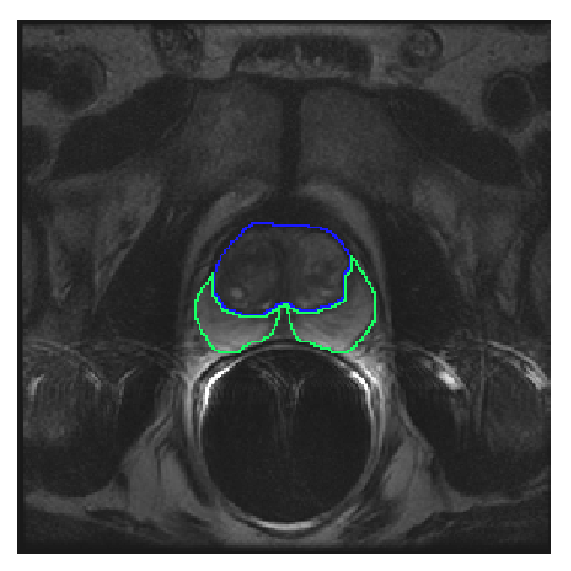
\includegraphics[width=.2\textwidth]{./images/mri/t2w/t2w_healthy.eps}}%
      \hfill%
      \subfigure[][\tiny CaP PZ]{%
        \label{fig:t2wcpz}%
        \includegraphics[width=.2\textwidth]{./images/mri/t2w/t2w_cancer_pz.eps}}%
      \hfill%
      \subfigure[][\tiny CaP CG]{%
        \label{fig:t2wccg}%
        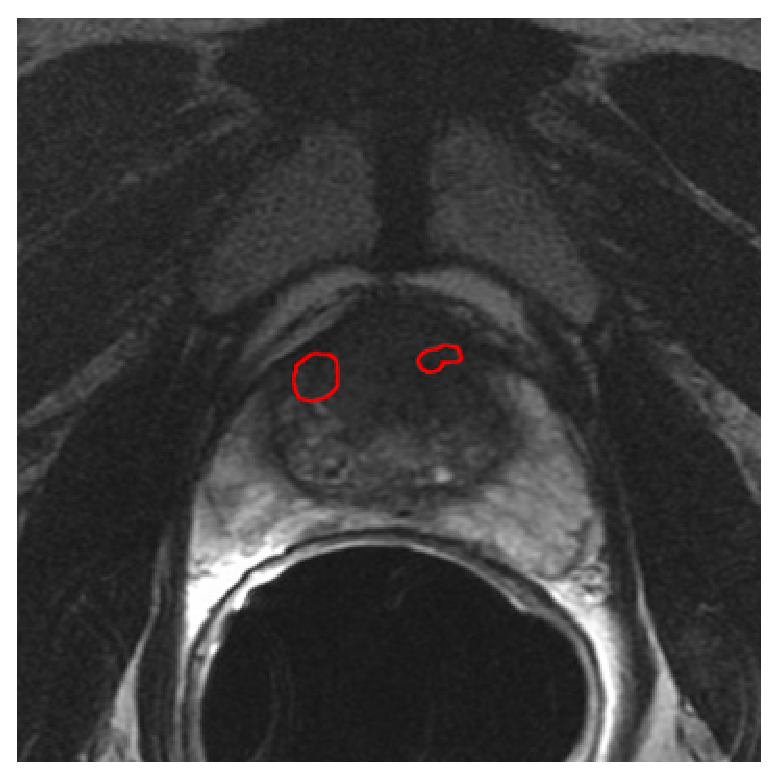
\includegraphics[width=.2\textwidth]{./images/mri/t2w/t2w_cancer_cg.eps}}%
      \hspace*{\fill}%
      \label{fig:t2w}%
    \end{figure}
  \end{block}
  \begin{redblock}{\small Features for CaP}\footnotesize
    \begin{itemize}
    \item Low-SI \& shape description 
    \end{itemize}
  \end{redblock}
\end{frame}

\subsection{MRI modalities}

\setcounter{subfigure}{0}% Reset subfigure counter

\begin{frame}
  \frametitle{Introduction}
  \framesubtitle{MRI modalities}
  \begin{block}{\small DCE MRI}
    \begin{figure}%
      \centering
      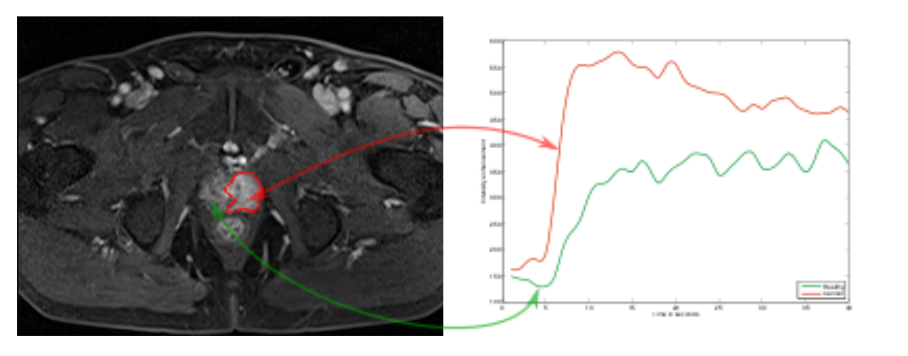
\includegraphics[width=.7\textwidth]{./images/mri/dce/dce_cancer_healthy_information.eps}
      \label{fig:dce}%
      \caption{{\color{green}Green}: healthy - {\color{red}Red}: CaP}
    \end{figure}
  \end{block}
  \begin{redblock}{\small Features for CaP}\footnotesize
    \begin{itemize}
    \item Faster wash-in, wash-out, time-to-peak enhancement
    \item Higher integral under the curve, max SI
    \end{itemize}
  \end{redblock}
\end{frame}

\begin{frame}
  \frametitle{Introduction}
  \framesubtitle{MRI modalities}
  \begin{block}{\small DW MRI - ADC}
    \begin{figure}%
      \centering
      \hspace*{\fill}%
      \subfigure[][\tiny DW MRI]{%
        \label{fig:dw}%
        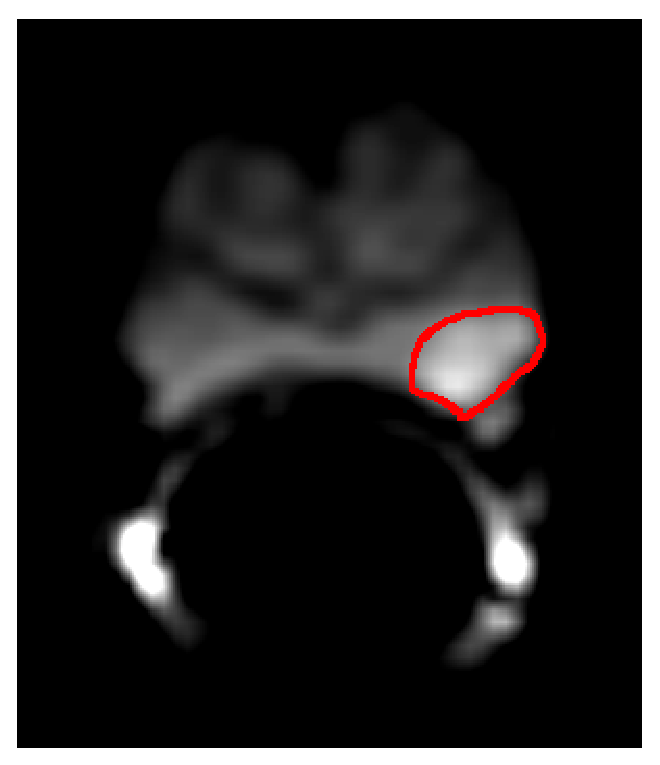
\includegraphics[width=.2\textwidth]{./images/mri/dwi/dwi_cancer.eps}}%
      \hfill%
      \subfigure[][\tiny ADC]{%
        \label{fig:adc}%
        \includegraphics[width=.2\textwidth]{./images/mri/dwi/adc_cancer.eps}}%
      \hspace*{\fill}%
      \label{fig:dwadc}%
    \end{figure}
  \end{block}
  \begin{redblock}{\small Features for CaP}\footnotesize
    \begin{itemize}
    \item DW MRI - Higher SI
    \item ADC - Low-SI
    \end{itemize}
  \end{redblock}
\end{frame}

% \begin{frame}
%   \frametitle{Introduction}
%   \framesubtitle{Screening}
%   \begin{columns}
%     \column{.5\textwidth}
%     \begin{block}{\tiny T$_2$-W MRI}
%       \begin{figure}
%         \centering
%         \includegraphics[height=0.25\textheight]{.//t2w/t2w_cancer_pz.eps}
%       \end{figure}
%     \end{block}
%     \begin{block}{\tiny DCE MRI}      
%       \begin{figure}
%         \centering
%         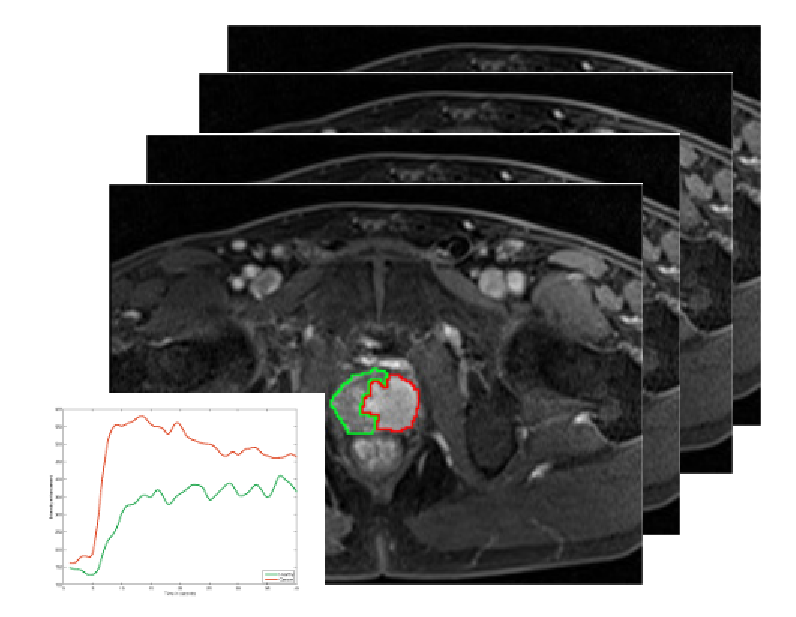
\includegraphics[height=0.25\textheight]{./figures/dce/dce_all.eps}
%       \end{figure}
%     \end{block}
%     \column{.5\textwidth}
%     \begin{block}{\tiny ADC MRI}
%       \begin{figure}
%         \centering
%         \includegraphics[height=0.25\textheight]{./figures/dwi/adc_cancer.eps}
%       \end{figure}
%     \end{block}
%     \begin{block}{\tiny MRSI}
%       \begin{figure}
%         \centering
%         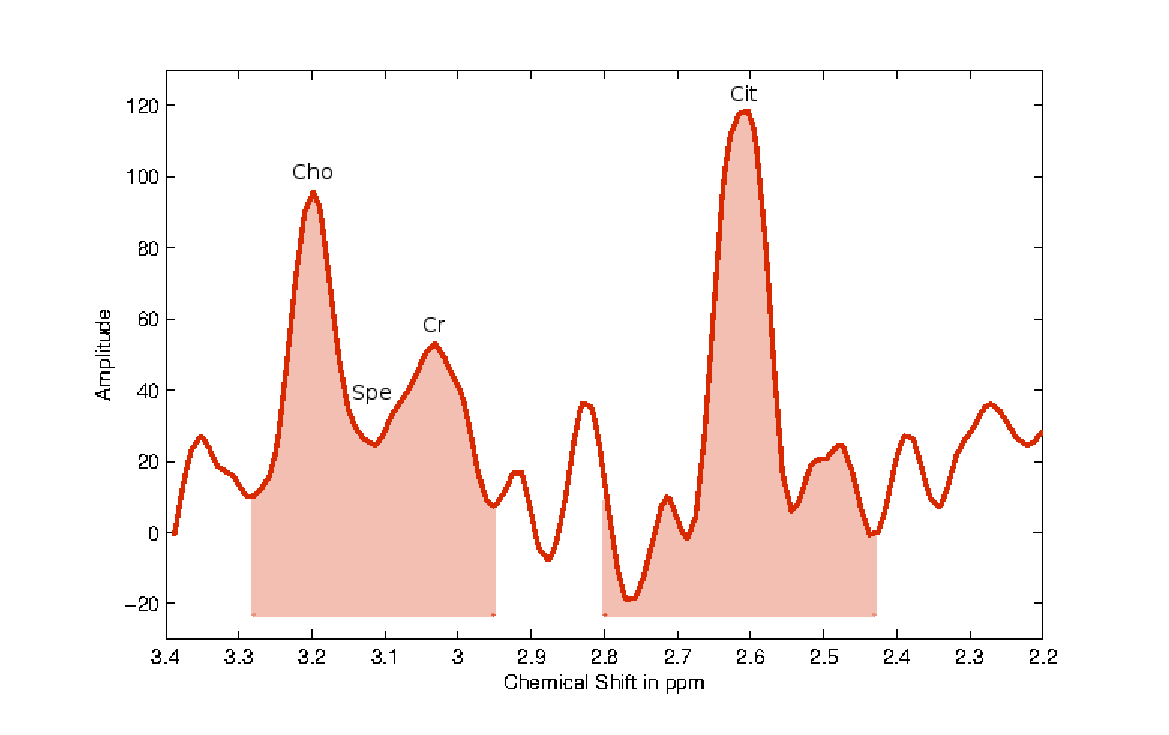
\includegraphics[height=0.25\textheight]{./figures/mrsi/mrsi_cancer.eps}
%       \end{figure}
%     \end{block}
%   \end{columns}
% \end{frame}

\subsection{Second subsection}

\begin{frame}
  \frametitle{A Kick-Ass Title}
  \framesubtitle{A Kick-Ass Title Subtitle}
  \begin{block}{Block environment}
    \begin{itemize}
    \item[\cross] Cross item
    \item[\tick] Tick item
    \end{itemize}
  \end{block}
  \begin{equation}
    \label{eq:eq1}
    f(x)=ax+b \ .
  \end{equation}
\end{frame}

\end{document}